\chapter{Preparation}
\label{sec:firststeps}

\section{Initial Researches}
Some research on the working principle of Alphasense \chem{NO_2} electrochemical sensor had to be made prior to the initialization of the mechanical and electrical sections of this project. The paper \cite{Hutton2011} on previous experiments conducted in Boston, United States of America was very helpful to get a first idea about how I could start building my project designed for \chem{NO_2} density measurements. In another paper about a research conducted in Zurich, Switzerland, \cite{Mueller2017} it is emphasized that it is quite expensive to build a gas pollutant measurement station sensitive to a certain gas and thus low-cost sensor stations play a very important role in collecting environmental data. \par 
My goal was to build a functioning circuit, to get meaningful data from it and to document the entire process of my project well, and the researches and the papers I read gave me even more motivation about how topical air pollution is and thus how important it is to try to build a low-cost air pollutant density measuring station and to collect useful environmental data.

\section{Getting a Better Understanding}
I had to read the application notes on the Alphasense webpage to get a better understanding of the inner structure as well as the pinout of the sensor and for this purpose, I began to study the documentation about the toxic sensors \cite{HowElectrochemicalGasSensorsWork}. As I started to understand which electrode of the sensor was responsible for which purpose, I began to get an idea of how I could build my own circuit, which would be able to supply enough current to the sensor and output voltage, linearly proportional to the concentration of the air pollutant, which in other words is the ppb level of \chem{NO_2} in the air. \par
Afterward, I started to read the documentation from Alphasense \cite{2009}, which gave me a starting point for the circuit. In Figure ~\ref{fig:A.1} you can see a circuit design for a three-electrode sensor. I was actually working with the sensor NO2-B43F, which is a four-electrode sensor, but this circuit schematic was nonetheless a good point to start building and testing the circuit.

\chapter{Putting Into Practice}

\section{Building the Initial Circuit}

\subsection{Hardware}
\subsubsection{Circuit Design}
In order to understand the circuit fully, we must first study the structure and the pinout of the NO2-B43F sensor. There are 4 electrodes of the electrochemical sensor: Working electrode, the reference electrode, the counter electrode, and the auxiliary electrode. The reference electrode holds the potential of the working electrode stable at a certain level, which is equal to the potential of the reference electrode itself. This potential must be fixed to ensure a stable outcome from the sensor and the circuit. The counter electrode must be able to supply enough current to the working electrode so that the current through the counter and working electrode can be translated and amplified to create the output voltage.\par
The A4 and B4 sensors have two sensing electrodes: The working electrode and the auxiliary electrode. The main purpose of the working electrode is to react to the \chem{NO_2} in the air and thus create a current flow proportional to the gas concentration. In other words, the working electrode responds to gas concentration whereas the auxiliary electrode does not respond to gas. The idea is to be able to correct for zero drifts using the auxiliary electrode output. It is thus recommended that at the beginning both electrode outputs are recorded (Working electrode and auxiliary electrode) rather than applying a correction directly.\par
The circuit in Figure ~\ref{fig:A.1}, in general, comprises of operational amplifiers, a couple of capacitors to reduce noise from the sensor and various resistors to get the desired gain from the operational amplifiers. On the left-hand side of the circuit, the NO2-B43F sensor is connected via 3 electrodes to the circuit. This schematic is for 3 electrode sensors like previously mentioned, so the auxiliary electrode is left out. The power connections of the operational amplifiers are also not shown, however they must be provided a regulated and high enough voltage to encompass the maxima of the output voltage. In addition to that, the power supply must be rated with high enough current to be able to supply the required current drawn by the counter electrode and the operational amplifiers themselves.\par
The circuit consists of 2 stages of amplifiers. The first stage is the control circuit, whose main objective is to supply the counter electrode with enough current so that the current required by the working electrode is met. The potential at the reference electrode, namely the reference voltage is connected to the inverting input of the operational amplifier. It is important that near to zero current is drawn from the reference electrode, so an op-amp with minimal input bias current is recommended. \cite{2009} \par 
Since the current control part of the circuit can already supply the counter electrode with enough current, the next step is to build the sensing part of the circuit, namely the current measuring stage. In this stage, the current through the counter and working electrode flows through the sensing resistor R\textsubscript{Load}, which in return creates a voltage on the inverting input of the second operational amplifier IC1. As it is mentioned before this current through R\textsubscript{Load} is linearly proportional to the gas concentration in the air. As a reminder, our main goal is to measure the amplitude of this current created by the working electrode, which gives us information about the concentration of \chem{NO_2}. The voltage difference between the inputs of IC1 is amplified (multiplied) by a very large number and is created on the output of IC1. However, this high voltage is fed back to the inverting input over the resistor R4, which increases the voltage on the inverting input and thus reduces the voltage difference between the inputs of the operational amplifier. As a result, the output voltage is reduced and so is the influence of the output on the inverting input voltage. This pendulum saturates at a specific voltage level, which is equal to the input voltage multiplied by a constant determined by the resistors R\textsubscript{Load} and R4. In this specific case the operational amplifier is being operated in inverting configuration, since the input voltage is connected to the inverting input of the operational. amplifier. Therefore the constant i.e. the gain of the amplifier is equal to the following: \[A = \frac{V_{Out}}{V_{In}} = -\frac{R_4}{R_{Load}} \] \par
In conclusion, the control stage supplies the required current by the counter electrode to the sensor, which is created by the potential difference between the counter and working electrodes. The current then flows through the sensing resistor  R\textsubscript{Load} creating a voltage on the inverting input of IC1. This input voltage is then multiplied by the gain and in the end, creates the output voltage.

\subsubsection{Microcontroller}
For this project, I decided to use an Arduino Uno board, since it is inexpensive and easy to use. I used a 12 Volts 1 Amp wall adapter for the power supply of the Arduino board. The Arduino board has 5V and 3.3V voltage regulator onboard. Since this circuit does not consist any component which requires high current, the voltage regulation from 12 Volts down to 5 Volts does not dissipate any excessive heat. \par
I put all the parts depicted in the circuit design together on a breadboard. For the power supply needed for the operational amplifiers I simply used the $5V$ and $GND$ power supply lines of the Arduino Uno board. The output of IC1 is connected to the analog input $A0$ on the board, which makes the voltage level readings possible. 


\subsection{Software}
The Arduino Uno board is simply an I/O device with several outputs and input pins. Through programming, via the Arduino Integrated Development Environment (IDE) these pins can be accessed and thus works as an interface between the circuit and the computer. It is capable of reading the voltage connected to its input, sending it to the computer via serial communication. These values sent from the Arduino are then displayed on the computer screen via the Arduino Integrated Development Environment (IDE). But in order to let the Arduino board know which data to send and at which frequency, we first have to program it using the same Arduino IDE.\par
Arduino can supply voltage and read voltage inputs up to 5 Volts. Analog inputs of the Arduino divide the continuous voltage range from 0 Volts to the analog reference voltage into 1024 discrete steps while digital outputs with Pulse Width Modulation (PWM) feature can supply 1024 different levels of voltage from 0 Volts up to a maximum of 5 Volts. Digital outputs without this feature can only supply either 0 Volts (LOW) or 5 Volts (HIGH). For this purpose, I connected the output pin of the operational amplifier in the last stage to one of the analog inputs on the Arduino. This way I could read the voltage level on the output of the operational amplifier at a high frequency (9600 bits per second) and thus get enough data to plot the output signal with sufficient resolution. \par
For this reason, I wrote a simple Arduino code using the Arduino IDE. This code consists of two standard main functions, namely $setup()$ and $loop()$. The $setup()$ function is called once when the sketch starts and runs only once after each powerup or reset of the Arduino board. Afterward, the $loop$ function is called and loops consecutively as the name suggests. In $setup()$ the serial communication speed, at which the microcontroller Atmega328p of the Arduino Uno is going to communicate with the computer, set with the function $Serial.begin()$ at 9600 bits per second. In $loop$ the function $Serial.print()$ is then used to print the voltage values on the serial monitor or on the serial plotter. For testing purposes, it is recommended to use the serial monitor embedded in the Arduino IDE, since it is sufficient to show the voltage values at the analog pin on the computer. Alternatively, the serial plotter, again embedded in the Arduino IDE, can be used to plot the data and thus to create a sample-voltage graph. At the end of the code, I added the $delay()$ function, which "[p]auses the program for the amount of time (in milliseconds) specified as parameter." \cite{delay}. In the code, I have set the parameter equal to 50 resulting in a 50 milliseconds delay before acquiring the next value. This way it becomes more pleasant to read the data printed on the serial monitor.

\subsection{Discussion}
This design was a success in terms of testing the sensor and the circuit. The values printed on the serial monitor showed us that the sensor reacted to the \chem{NO_2} concentration in the air. However, it was lacking protection against electrical noise and the values were not similar to the nominal values which were determined with the help of the Individual Sensor Board (ISB) from Alphasense. Most importantly the auxiliary electrode was left out, which is why a correction for zero drifts was impossible with this circuit design alone. An improvement of the circuit was needed for better results, namely for the output data to get closer to the nominal values of the ISB circuit. Therefore I started to study and eventually build the circuit explained in the next section.  


\section{Realising the Last Circuit}
\subsection{Hardware}
The circuit in Figure~\ref{fig:A.2} consists of 3 operational amplifier ICs, a couple of capacitors to reduce noise from the power supply and various resistors to get the required output voltage to input voltage ratio from each operational amplifier. Unlike the previous circuit design, the auxiliary electrode is included in this schematic, which will be helpful in the future to make zero drift corrections through programming and thus better results outputted from the circuit. Additionally, the subcircuit for the low-dropout DC linear voltage regulator $MCP1702T25$ is also depicted in detail. Lastly, the power supply subcircuit of the operational amplifiers is included.

\subsubsection{Main Circuit}
This design consists of two branches which lead to two different outputs. The working electrode of the sensor leads to the first branch and thus the first output $O/P1$, while the auxiliary electrode leads to the second output $O/P2$. However, both branches are identical copies of each other. The main reason to build two identical copies of a branch is to separate the working and the auxiliary electrode from each other in order to avoid any interference between the two electrodes. Like mentioned before, the auxiliary electrode does not react to \chem{NO_2} and thus the voltage level at $O/P2$ must not change depending on the \chem{NO_2} density in the air. Additionally, it is to notice that two different operational amplifier ICs, namely two separate $LT6011$ chips are used in order to separate the two branches better. The operational amplifiers $U4A$ and $U4B$ constitutes one $LT6011$, while $U1A$ and $U1B$ constitutes the second IC. The last operational amplifier $U2$ is the IC $TLV2211$ which consists of only one operational amplifier. Although the two different ICs have similar features, $TLV2211$ is more efficient in power consumption and spatial terms since the $LT6011$ has a bigger packaging than the $TLV2211$ and consumes more energy. \cite{TLV2211} \cite{LT6011}\par
The first stage of the circuit is the same as the initial design explained in the previous section. The only difference is that the capacitor $C2$ in the initial design is left out in this schematic, which is not necessary for this operational amplifier. \cite{2009} Since this stage is explained in detail in the previous section, it is not needed to explain it again. \par 
After the first stage, the circuit divides into 2 branches through the working and the auxiliary electrodes of the sensor. Like mentioned before these branches are identical, so it is more meaningful to explain only the branch starting from the working electrode in detail as the same logic can be applied to the branch starting from the auxiliary electrode leading to $O/P2$.\par
$V_{mid}1$ is directly connected to the output of the voltage regulator and has a potential of 2.5 Volts, which is explained in the next section in detail. The current flowing through $R15$ creates a voltage difference between its two ends, namely the working electrode and the inverting input of $U4B$. Since the potential of the working electrode is equal to the reference electrode and thus to 2.5 Volts, the voltage on the inverting input is higher than 2.5 Volts and thus is also higher than $V_{mid}1$, which is connected to the non-inverting input of the operational amplifier. As the \chem{NO_2} concentration gets higher, the current flowing through $R15$ becomes greater. For this reason the voltage difference between the two inputs of $U4C$ changes linearly proportional to the ppb level of \chem{NO_2}. This voltage difference gets amplified through $U4B$. The amplified voltage created at the output of $U4A$ goes into the inverting input of the last operational amplifier on this branch $U2$. The voltage level on the non-inverting input of $U2$ is determined by the voltage divider circuit consisting of $R29$, $R30$, $R8$, $R7A$ and $R9$. For this reason, the voltage level of the non-inverting input is between 0 and 2.5 Volts. The voltage difference between the inputs of $U2$ is then multiplied by the gain of the operational amplifier, which is determined by the resistors $R6A$, $R4$ and $R3$. The same formula used for the earlier stage can be applied here, while the input resistor $R_{in}$ is $R6A$ and the value of the feedback resistor $R_f$ is equal to the sum of the values of $R4$ and $R3$, as they are connected in series. The voltage outputted from $U2$ is approximately equal to the output voltage since the resistor $R1$ has a much greater value than $R3$ and has a negligible effect on the output voltage. $R1$ and the capacitor $C3$ are against noise at the output of the circuit $O/P1$.\par 
In conclusion, the working principle of the main circuit can be summarized as follows: The voltage output at $O/P1$ is the current created through the voltage difference between the working and the counter electrode translated to a voltage with the help of resistors and amplified through 2 stages of operational amplifiers.\par 
The voltage levels at $O/P1$ and $O/P2$ are supplied to the analog inputs of the Arduino board and then gets printed on the computer. Since the voltage at $O/P1$ is a translation of the working electrode and the voltage at $O/P2$ is a translation of the auxiliary electrode, both outputs can be used at the same time for noise reduction and zero drift correction which leads to more reliable results than the data outputted using the initial design.


\subsubsection{Voltage Regulator Subcircuit}
On the bottom left corner, the voltage regulator subcircuit is to be observed. This part of the schematic consists of a low-dropout DC linear voltage regulator $MCP1702T25$, a Zener diode with 6.8V Zener voltage, an electrolytic capacitor, and various resistors and ceramic capacitors. The $MCP1702T25$ receives the input voltage at its $V_{in}$ pin and translates it to a regulated 2.5V potential level at $V_{out}$. The last pin depicted as $Adj$ in the schematic is simply connected to $GND$. The input voltage at $V_{in}$ is also regulated with an external voltage regulator $L7806CV$, which converts the 12V outputted from the wall adapter down to 6 Volts. The Zener diode $D2$ cuts off any excess voltage higher than 6.8 Volts by shorting $V_{in}$ with $GND$. Therefore it is dismissable since the 6 Volts input voltage is outputted from the $L7806CV$ voltage regulator and is less than 6.8 Volts at all times. The resistor $R16$ is connected to an unregulated voltage supply, and therefore is also not necessary in our circuit. On the output side of the voltage regulator the resistors $R21$, $R19$, $R27$ and $R28$ constitutes a voltage divider circuit which creates the voltage level depicted as $V_{off}1$. $V{pot}1$, $V{pot}2$, $V{ce}1$ and $V{mid}1$ are all connected directly to $V{out}$ and thus have the same 2.5V potential. The capacitors $C5$, $C12$ and $C13$ cuts out the AC part of the input and output voltages and thus reduces the overall noise ratio at the outputs $O/P1$ and $O/P2$.

\subsubsection{Power Supply of the Operational Amplifiers}

The operational amplifiers depicted as $U1C$ and $U4C$ are connected to the 6V regulated voltage level outputted from the $L7806CV$. The capacitors $C2$ and $C8$ are in parallel to the ICs and thus shorts the AC component of the input voltage while staying open for the DC section. This results in a more stabilized input voltage for the operational amplifier ICs and therefore reduces noise overall in the circuit. The single operational amplifier IC $TLV2211$ is also connected in parallel to the two $LT6011$ ICs, which is not depicted in this circuit schematic.

\subsubsection{SD Card Module}
An SD card module has been added to the circuit in order to save the concentration data supplied by the circuit. Six connections between the SD card module and the Arduino board are needed for a successful communication between the two. The $V_cc$ pin is connected to the $5V$ or the $3V3$ power supply line of the Arduino board, while the $GND$ pins of both module and the board are connected together to ensure a common ground. The $MOSI$ pin is connected to the eleventh pin, the $MISO$ pin is connected to the twelfth pin and the $SCK$ pin is connected to the thirteenth pin of the Arduino board. The $CS$ pin is connected to the fourth digital I/O pin of the Arduino board. Lastly, there is an LED connected to the fifth digital I/O pin of the board which indicated the status of the SD card module. The details of saving data into the SD card are explained further in the next section. 


\subsection{Software}
The previous software for the initial circuit design is developed and some new features are added to the code (please see ~\ref{code:label}). The recent Arduino code can not only show the voltage levels at $O/P1$ and $O/P2$ on the serial monitor or the serial plotter but also saves every incoming data into an SD card provided with a time stamp.\par 
First of all the programming libraries needed for providing a time stamp and saving the data into an SD card are included at the beginning of the Arduino code; namely $TimeLib.h$, $SPI.h$ and $SD.h$. Afterward comes the declaration of the two constants $TIME\_HEADER$ and $TIME\_REQUEST$. The latter is set to $7$ which is the ASCII bell character. The former is set to the character \textit{T}. For this reason, whenever a time stamp is provided to the Arduino board via serial communication, the header \textit{T} must be also provided at the start of the UNIX timestamp, which will then be recognized by the Arduino microcontroller as a time stamp and attached to the incoming data from the circuit. After a time stamp has been provided to the microcontroller, the process of providing a time stamp for every succeeding incoming data is done automatically, since the microcontroller can track time beginning from the initialization of the sketch. For this reason, it is only needed once to provide a time stamp to the microcontroller via serial monitor. The parameter $chipSelect$ is set to \textit{4} since the $CS$ pin of the module is connected to the fourth pin of the board. \par
In the $setup()$ function the serial communication speed is set to 9600 bits per second. Since the incoming voltage levels are in millivolts, it is recommended to set the analog reference (which is set to 5 Volts as default) to the virtual ground of the circuit at 2.5 Volts (in reference to the common ground). For this purpose the function $analogReference()$ is called and its input parameter is set to $EXTERNAL$. The analog reference pin $AREF$ of the Arduino board is thus connected to the 2.5V power supply line of the circuit, which sets the analog reference voltage to the same voltage level. The resolution of the data is therefore doubled since the reference voltage is halved.\par
The function $pinMode()$ is called in order to set the fifth pin of the board as $OUTPUT$, which drives the LED indicating the status of the module. A series of functions are called for the initialization of the SD card module: $setSyncProvider()$ sets the external time provider. \cite{Time} The function $processSyncMessage()$ sets the internal clock of the Arduino microcontroller to the time received on the serial port. This is done by receiving the time stamp sent via serial monitor and decoding the message. $Serial.find()$ searches for the letter \textit{T} in the message and decodes the rest of the message into time information using the function $Serial.parseInt()$. After the message is decoded and the time information is acquired, the internal clock of the microcontroller is set to the received time. Therefore the clock gets synchronized with the real-time and the microcontroller can attach time to the incoming data. Lastly the function $SD.begin()$ initializes the SD library and the module \cite{SD}, which returns a variable in boolean. If the initialization is a success, $true$ is returned and the message "Card Initialized" is printed on the serial monitor; and otherwise $false$ is returned and the message "Card failed, or not present" is printed. \par 
In $loop()$ function the serial communication is checked with the function $Serial.available()$ which returns a boolean. If $true$ is returned, the $processSyncMessage()$ is called and the time is set to the received UNIX time stamp. Afterward, the status of the time synchronization is checked by calling the function $timeStatus()$ which indicates if the time has been set. \cite{Time} If the synchronization is flawless the fifth pin is set to $HIGH$ and the indicator LED is powered on. Otherwise, the LED turns off and indicates an error concerning the synchronization. Afterward, a string called $dataString$ is created. This string is then set to a series of strings concatenated together, which contain data of the values of two outputs $O/P1$ and $O/P2$ as well as the date and time at which the data was received. After that the $datalog.txt$ file contained in the SD card is opened by calling $SD.open$ and setting its mode to $FILE\_WRITE$. This enables writing incoming data from the circuit onto the $datalog.txt$ file in the SD card. If the $datalog.txt$ is available for writing the string $dataString$ is written into the $datalog.txt$ file by calling the $dataFile.println$ function and is closed after $dataFile.close$ is called. After the save is completed the $dataString$ is printed on the serial monitor for testing purposes. If the file is unavailable the message "Error opening datalog.txt" is printed on the serial monitor. Lastly, a $delay()$ function with its input parameter set to $1000$ pauses the code for 1000 milliseconds, namely for one second. After the $delay()$ function is executed and exited the $loop()$ function starts again from the top and saves the next incoming data provided with time information.         

\subsection{Discussion}
Since the circuit has more resistor-capacitor pairs at the inputs and outputs of each operational amplifier, there is less noise contained in the output signal. Additionally, the auxiliary electrode was included in this circuit design, which protected the electrode from floating, unlike the previous design.

\chapter{Results}
The $Amplitude$ axes in Figures~\ref{fig:4.1} to ~\ref{fig:4.4} depicts the voltage level using a specific scale. Like mentioned before, the analog reference is 2.5 Volts and the maximum output value is 1023. Therefore the values on the $Amplitude$ axes must be multiplied by 2.5 and divided by 1023 to obtain the values in Volts. Another multiplication with 1000 results in values in mV. \par    
The outputted data from the circuit were at the beginning unstable. The noise ratio contained in the signal was very high compared to the signal outputted from the ISB board. In Figure~\ref{fig:4.1} the output signal of my circuit with high noise ratio can be examined in detail. The sampling frequency is 200Hz and the noise frequency is approximately 50Hz. After some research, I found out that the noise may be caused by a noisy USB port supply of the computer. After plugging the laptop in instead of using it on battery power, the noise ratio dropped significantly and the outputted signals were comparable to the ISB values. In Figure~\ref{fig:4.2} it is to be noticed that the noise ratio drops dramatically beginning from approximately 260. sample. At this point, the laptop was plugged in and thus the signal got significantly more stable. \par 
After plugging the wall adapter in, and thus supplying power to the Arduino board, the SD Module and the main circuit; there is a stabilization time for the sensors to reach saturated results. The duration of this process varies from 10 minutes up to 2 hours for NO2-B43F sensors depending on the time passed after the last use. \cite{FAQs} In Figure~\ref{fig:4.3} the stabilization process of the sensors are depicted. The sampling frequency is equal to 1Hz, namely, the sampling occurs every second. It is to notice that the stabilization speed is different for different sensors, but the saturation level is approximately equal for each sensor under the same environmental conditions. Both $O/P1$ and $O/P1 ISB$ values saturated at approximately 94, which is close to 230 mV. With the help of the graph displayed in Figure~\ref{fig:4.5} the voltage level can be converted into the ppb level of \chem{NO_2} in the environment. For this occasion, the density of \chem{NO_2} is equal to 150 ppb. \par 
Lastly the Figure~\ref{fig:4.4} depicts the sensor reaction to air flow perpendicular to the sensor surface. The air flow was initiated at the 25. sample and was terminated at the 31. sample. It is to be noticed that there is no significant difference between the sensor reactions. This demonstrates the success of the circuit board and proves the reconstructability of the sensor unit.  



%The outputted data from the circuit were at the beginning unstable. The signal-to-noise ratio was too low compared to the values from the ISB circuit. After noticing the pattern of the noise ratio contained in the signal, I started to make a deeper examination of the signal. In Figure~\ref{fig:4.1} the signal can be observed in high resolution, namely the sampling rate is 5 milliseconds per sample, or 200Hz. After a brief research on electrical noise, I found out that the problem was caused by the USB VBUS supply of the laptop, which is connected to the Arduino board.   





	\begin{figure}
		\begin{center}
		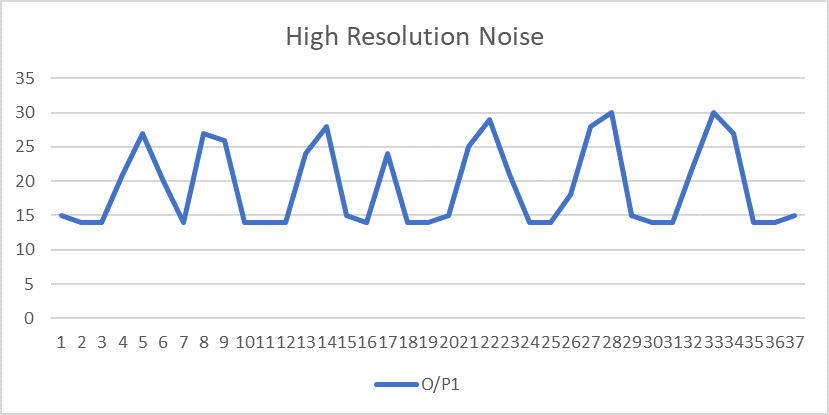
\includegraphics[width=1\textwidth]{Pics/3}
		\caption{Signal with High Noise Ratio (High Resolution)}
		\label{fig:4.1}
		\vspace{2cm}
		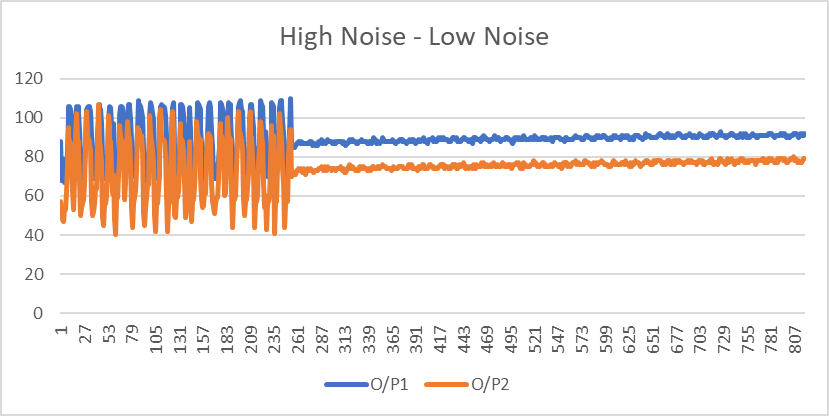
\includegraphics[width=1\textwidth]{Pics/1}
		\caption{Output Signal Comparison with High and Low Noise Ratio}
		\label{fig:4.2}
		\vspace{2cm}
	\end{center}
	\end{figure}
		\newpage
		\begin{figure}
			\begin{center}
				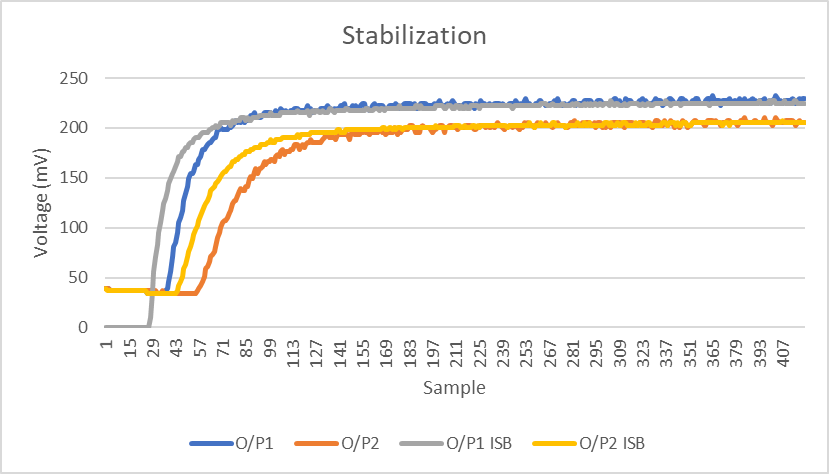
\includegraphics[width=1\textwidth]{Pics/4}
				\caption{Stabilization Process}
				\label{fig:4.3}
				\vspace{2cm}
				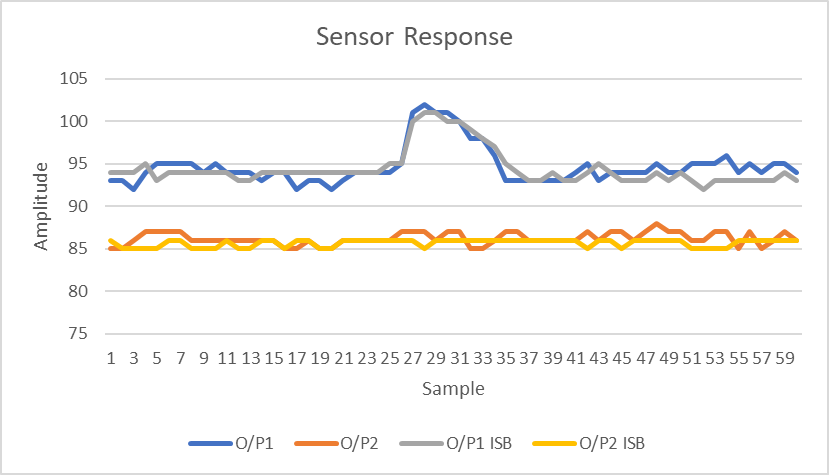
\includegraphics[width=1\textwidth]{Pics/2}
				\caption{Reaction Comparison of Both Circuits}
				\label{fig:4.4}
			\end{center}
		\end{figure}
	\newpage
	\begin{figure}
		\begin{center}
	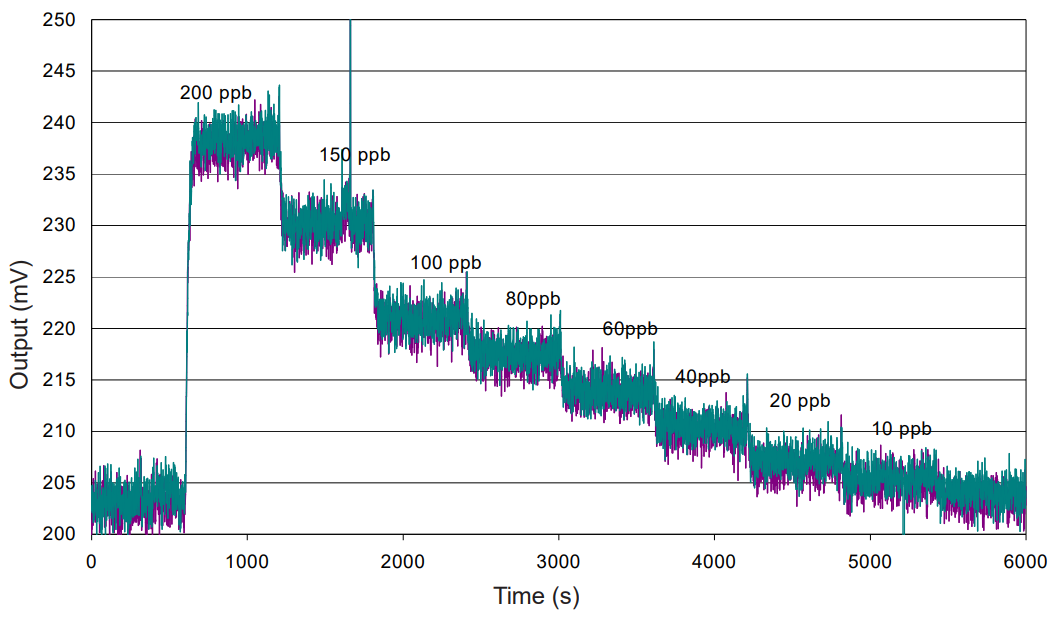
\includegraphics[width=1\textwidth]{Pics/9}
	\caption{Response to 200 ppb \chem{NO_2} \cite{Datasheet}}
	\label{fig:4.5}
	\medskip		
\end{center}
\end{figure}